% Version 1.2 of SN LaTeX, November 2022
%
% See section 11 of the User Manual for version history 
%
%%%%%%%%%%%%%%%%%%%%%%%%%%%%%%%%%%%%%%%%%%%%%%%%%%%%%%%%%%%%%%%%%%%%%%
%%                                                                 %%
%% Please do not use \input{...} to include other tex files.       %%
%% Submit your LaTeX manuscript as one .tex document.              %%
%%                                                                 %%
%% All additional figures and files should be attached             %%
%% separately and not embedded in the \TeX\ document itself.       %%
%%                                                                 %%
%%%%%%%%%%%%%%%%%%%%%%%%%%%%%%%%%%%%%%%%%%%%%%%%%%%%%%%%%%%%%%%%%%%%%

%%\documentclass[referee,sn-basic]{sn-jnl}% referee option is meant for double line spacing

%%=======================================================%%
%% to print line numbers in the margin use lineno option %%
%%=======================================================%%

%%\documentclass[lineno,sn-basic]{sn-jnl}% Basic Springer Nature Reference Style/Chemistry Reference Style

%%======================================================%%
%% to compile with pdflatex/xelatex use pdflatex option %%
%%======================================================%%

%%\documentclass[pdflatex,sn-basic]{sn-jnl}% Basic Springer Nature Reference Style/Chemistry Reference Style


%%Note: the following reference styles support Namedate and Numbered referencing. By default the style follows the most common style. To switch between the options you can add or remove “Numbered” in the optional parenthesis. 
%%The option is available for: sn-basic.bst, sn-vancouver.bst, sn-chicago.bst, sn-mathphys.bst. %  
 
%%\documentclass[sn-nature]{sn-jnl}% Style for submissions to Nature Portfolio journals
%%\documentclass[sn-basic]{sn-jnl}% Basic Springer Nature Reference Style/Chemistry Reference Style
\documentclass[sn-mathphys,Numbered]{sn-jnl}% Math and Physical Sciences Reference Style
%%\documentclass[sn-aps]{sn-jnl}% American Physical Society (APS) Reference Style
%%\documentclass[sn-vancouver,Numbered]{sn-jnl}% Vancouver Reference Style
%%\documentclass[sn-apa]{sn-jnl}% APA Reference Style 
%%\documentclass[sn-chicago]{sn-jnl}% Chicago-based Humanities Reference Style
%%\documentclass[default]{sn-jnl}% Default
%%\documentclass[default,iicol]{sn-jnl}% Default with double column layout

%%%% Standard Packages
%%<additional latex packages if required can be included here>

\usepackage{graphicx}%
\usepackage{multirow}%
\usepackage{amsmath,amssymb,amsfonts}%
\usepackage{amsthm}%
\usepackage{mathrsfs}%
\usepackage[title]{appendix}%
\usepackage{xcolor}%
\usepackage{textcomp}%
\usepackage{manyfoot}%
\usepackage{booktabs}%
\usepackage{algorithm}%
\usepackage{algorithmicx}%
\usepackage{algpseudocode}%
\usepackage{listings}%
%%%%

%%%%%=============================================================================%%%%
%%%%  Remarks: This template is provided to aid authors with the preparation
%%%%  of original research articles intended for submission to journals published 
%%%%  by Springer Nature. The guidance has been prepared in partnership with 
%%%%  production teams to conform to Springer Nature technical requirements. 
%%%%  Editorial and presentation requirements differ among journal portfolios and 
%%%%  research disciplines. You may find sections in this template are irrelevant 
%%%%  to your work and are empowered to omit any such section if allowed by the 
%%%%  journal you intend to submit to. The submission guidelines and policies 
%%%%  of the journal take precedence. A detailed User Manual is available in the 
%%%%  template package for technical guidance.
%%%%%=============================================================================%%%%

%\jyear{2021}%

%% as per the requirement new theorem styles can be included as shown below
\theoremstyle{thmstyleone}%
\newtheorem{theorem}{Theorem}%  meant for continuous numbers
%%\newtheorem{theorem}{Theorem}[section]% meant for sectionwise numbers
%% optional argument [theorem] produces theorem numbering sequence instead of independent numbers for Proposition
\newtheorem{proposition}[theorem]{Proposition}% 
%%\newtheorem{proposition}{Proposition}% to get separate numbers for theorem and proposition etc.

\theoremstyle{thmstyletwo}%
\newtheorem{example}{Example}%
\newtheorem{remark}{Remark}%

\theoremstyle{thmstylethree}%
\newtheorem{definition}{Definition}%

\raggedbottom
%%\unnumbered% uncomment this for unnumbered level heads

\begin{document}

\title[Article Title]{Supplementary Material for ``Developing Comprehensive Annotation Guidelines and a Corpus of Risk of Bias Assessment for Rehabilitation: A Methodological Approach''}

%%\pacs[JEL Classification]{D8, H51}

%%\pacs[MSC Classification]{35A01, 65L10, 65L12, 65L20, 65L70}

\maketitle


%%%%%%%%%%%%%%%%
%% Background %%
\section{Annotation Guidelines}
\label{sec:guidelines}
%
In each of the following subsections, we describe the annotation guidelines for the signalling questions using the instructional placards developed through consultation with RoB assessment and natural language processing experts.

\textcolor{red}{include a generic description about the colours, logos, shapes and flowchart elements in the placards here...}
%
%
%
\subsection{Signalling question: 2.3}
%
For annotation instructions for this signalling question, ``Were there deviations from the intended intervention that arose because of the trial context?'' follow the Flowchart~\ref{fig:2_3}.

\begin{figure}
    \centering
    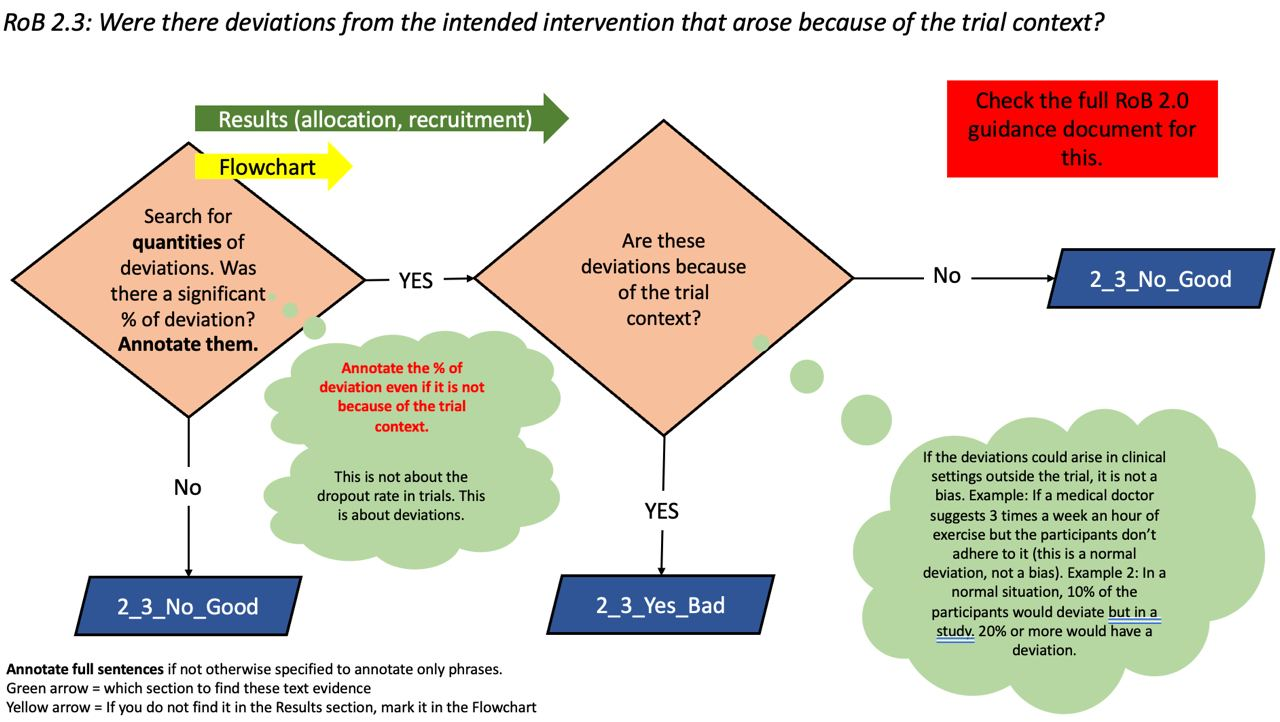
\includegraphics[width=\textwidth]{figures/2_3.jpg}
    \caption{Annotation instructions for the RoB 2.3 signalling question.}
    \label{fig:2_3}
\end{figure}
%
%
%
\subsection{2.3}
%
%
%
%%===========================================================================================%%
%% If you are submitting to one of the Nature Portfolio journals, using the eJP submission   %%
%% system, please include the references within the manuscript file itself. You may do this  %%
%% by copying the reference list from your .bbl file, paste it into the main manuscript .tex %%
%% file, and delete the associated \verb+\bibliography+ commands.                            %%
%%===========================================================================================%%

\bibliography{sn-bibliography.bib}% common bib file
%% if required, the content of .bbl file can be included here once bbl is generated
%%\input sn-article.bbl


\end{document}
